\section{External Validity}

Sections 3--5 are on synthetic graphs with a synthetic error knob. Is
the picture real? We stress it three ways: a genuine, cheap predictor on
a real request trace (§6.1); the six real-world graphs (§6.2); and
whether \emph{learning} the predictor changes anything (§6.3).

\subsection{A real, cheap predictor}

We replace the synthetic error knob with the cheapest realistic
predictor: last-window historical statistics. Real Wikipedia daily
pageviews give a live day (the truth) and earlier days (a 1-, 7-, or
30-day-stale forecast), so the prediction error is genuine temporal
drift; we map the trace onto a fixed serving topology and consume the
forecast through the degree route (MPD) (\textbf{Figure 7};
\texttt{docs/REAL\_PREDICTOR.md}).

\begin{figure}
\centering
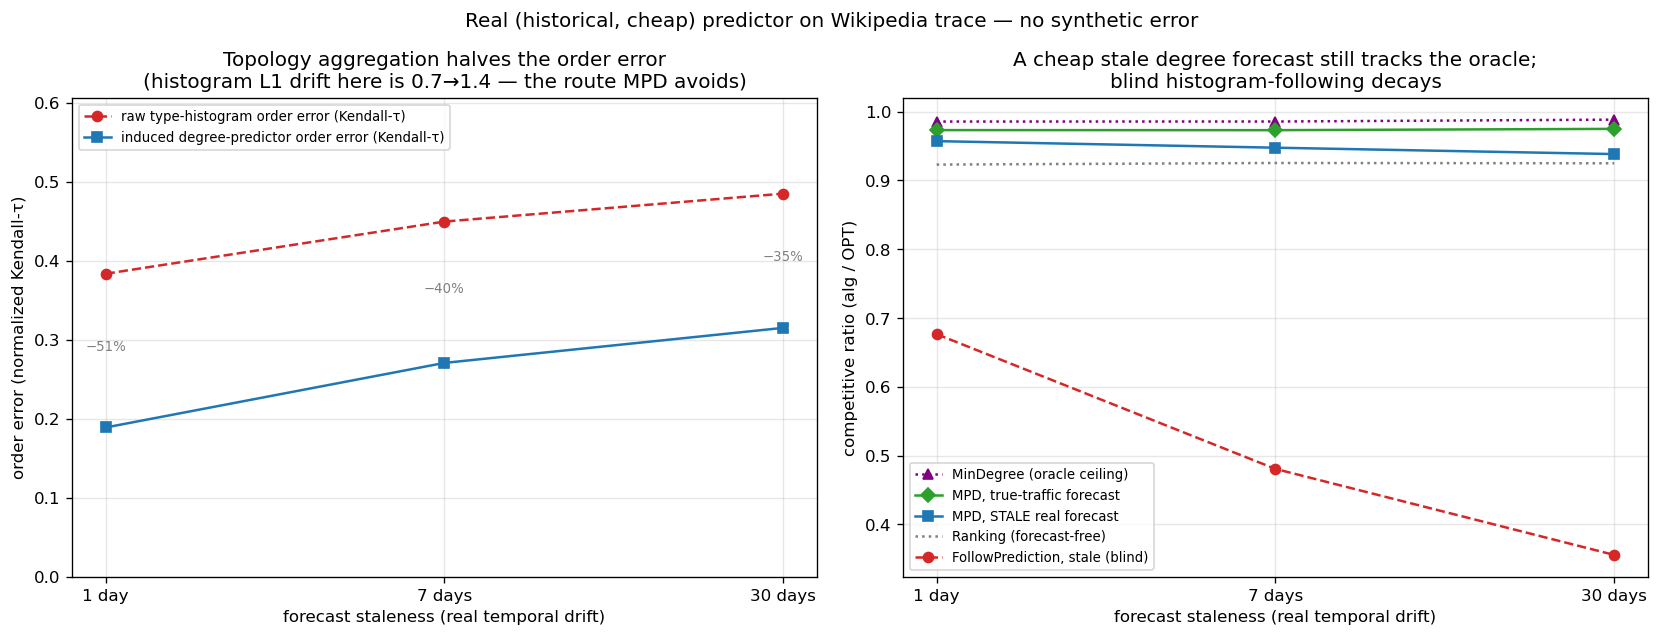
\includegraphics[width=0.8\linewidth,height=\textheight,keepaspectratio,alt={A cheap historical-count predictor on the Wikipedia trace: near-oracle ratio at every staleness level, never below the advice-free floor.}]{../../results/real_predictor.png}
\caption{A cheap historical-count predictor on the Wikipedia trace:
near-oracle ratio at every staleness level, never below the advice-free
floor.}
\end{figure}

Three facts emerge, all favorable and all honest. First, \textbf{the
cost premise does not bite}: the predictor is a linear-time count
(\(\mu = A\,p\) over historical frequencies), \(0.108\) ms per instance
--- about \(2\%\) of the cost of computing \(\mathrm{OPT}\) once --- not
an ML inference. Second, \textbf{the benefit is real, partial, and never
harmful}: a stale forecast captures \(27\%\)--\(68\%\) of the achievable
oracle gap (falling with staleness) and \emph{always} stays above the
forecast-free baseline (\(0.938\)--\(0.957\) vs \(0.923\)--\(0.925\),
even at 30 days). Third, and explaining why, \textbf{topology
aggregation makes the cheap predictor order-faithful}: the induced
degree predictor's order error is only Kendall-\(\tau\approx
0.19\)--\(0.32\), roughly \emph{half} the raw type-histogram's
(\(0.38\)--\(0.49\)) --- and since MPD depends only on order (Section
4), the aggregated degree route survives real drift. Consuming the
\emph{same} stale forecast through the raw histogram instead is
catastrophic: blind FollowPrediction collapses to \(0.68\to0.36\), far
below the \(\approx0.92\) baseline --- exactly what the robust
algorithms of Sections 3 and 5 are for.

\subsection{Six real-world graphs}

We re-run the degree-prediction roster of Section 3 on the six
Network-Repository graphs (two Facebook social, two C. elegans
biological, two economic input-output), across the same quality columns,
with 95\% CIs (\textbf{Figure 8};
\texttt{docs/REALWORLD\_ROBUSTNESS.md}).

\begin{figure}
\centering
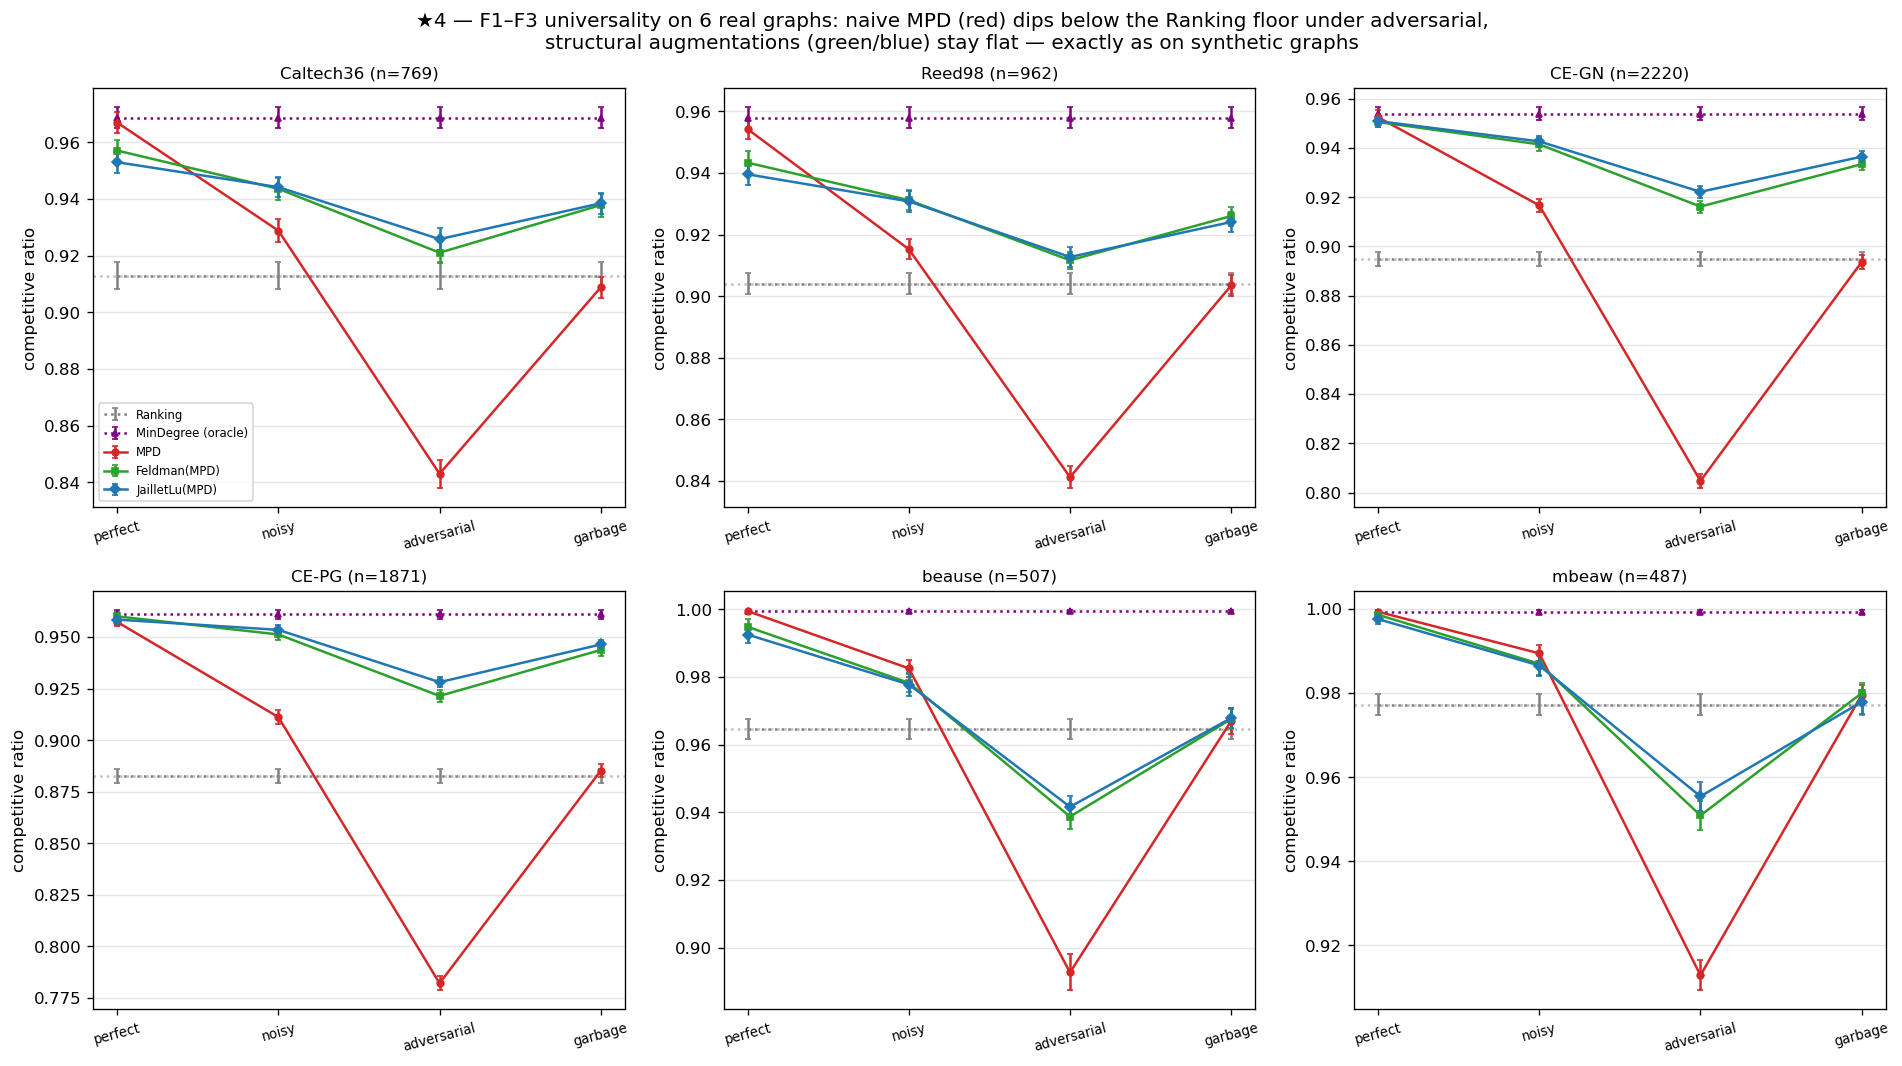
\includegraphics[width=1\linewidth,height=\textheight,keepaspectratio,alt={The six real-world graphs: unguarded following falls below the advice-free floor on every graph, and the augmentation restores safety --- the benchmark's findings are universal, not generator artifacts.}]{../../results/realworld_robustness.png}
\caption{The six real-world graphs: unguarded following falls below the
advice-free floor on every graph, and the augmentation restores safety
--- the benchmark's findings are universal, not generator artifacts.}
\end{figure}

The two load-bearing findings are universal. \textbf{F1 holds on all six
graphs}: naive MPD fed an adversarial predictor falls \emph{below} the
Ranking floor everywhere --- by \(0.07\) (Caltech36: \(0.843<0.913\)) to
\(0.11\) (CE-PG: \(0.782<0.883\)). **F3 is universal and

confirms its own logic**: the consistency upside (best prediction
algorithm at perfect advice, over the floor) is small everywhere (mean
\(+0.049\); range \(+0.022\)--\(+0.077\)), and it is \emph{smallest
exactly where the baseline is strongest} --- the two dense economic
graphs, with Ranking already \(0.965\)/\(0.977\), give the tiniest
upsides (\(+0.035\)/\(+0.022\)).

The structural-robustness finding \textbf{F2 holds qualitatively on all
six} (the augmentations are always less sensitive to prediction quality
than naive MPD) and \emph{strictly} on the four social/bio graphs
(augmentation spread \(0.22\)--\(0.29\times\) MPD's); on the two dense
economic graphs the protection is only \emph{partial} --- the
augmentation cushions the adversarial drop (beause: \(0.939\) vs naive
MPD's \(0.893\)) but cannot fully clear the unusually high \(0.965\)
floor, dipping \(\approx0.03\) below it (spread ratio
\(0.53\)--\(0.55\)). This econ boundary is instructive rather than a
failure: those graphs are so dense that matching is nearly trivial
(Ranking \(\approx0.97\), MinDegree \(=1.00\)), so there is neither
upside to capture (F3) nor much downside to protect --- the mechanisms
compress together

where robustness does not matter. Finally, F4 is \emph{dramatic} here:
the worst-case-designed Feldman/Jaillet--Lu are the weakest advice-free
entries on the econ graphs (\(0.73\)--\(0.77\)), and the MPD
augmentation lifts them to \(0.99\) --- a \(+0.26\) rescue.

\subsection{\texorpdfstring{Does \emph{learning} the predictor help? A
negative
result}{Does learning the predictor help? A negative result}}

Because MPD consumes the predictor only through its order (Section 4),
one might train the predictor with an order-aware (rank) loss rather
than regression. We test this and report an honest negative
(\texttt{docs/RANK\_LEARNING\_M0\_M3.md}). With \emph{deliberately
divergent} synthetic features --- one carrying magnitude, one carrying
order --- rank-training does beat regression sharply (matching ratio
\(0.989\approx\) oracle vs \(0.974\), with rank-training having
\emph{worse} regression error but better order). But the advantage is
gated by two things that both vanish in practice: it is zero when
features do not induce an order/magnitude divergence and zero on easy
instances (F3 again), peaking at only \(+1.3\%\) on synthetic graphs;
and, decisively, \textbf{on real temporal features it disappears} ---
trained on lagged counts from real serving traces, the rank- and
regression-trained predictors produce \emph{identical} order
(Kendall-\(\tau\) \(0.126\) vs \(0.126\)) and identical matching ratio,
across every topology and

lag we tried. The dissociation that powers order-aware training is a
property of engineered features, not of realistic ones. The lesson
reinforces the thesis: once a predictor is order-faithful --- which a
cheap historical count already is (§6.1) --- neither a better algorithm
nor a better-trained predictor buys much on average-case matching.

\subsection{Summary}

On real predictors, real graphs, and a learned predictor, the same wall
stands: the advice-free baseline is near-optimal, unguarded following is
unsafe, and predictions buy downside protection rather than performance.
Having established the wall empirically across every setting we could
reach, we now prove it is necessary.
